



\begin{concept}{Ableitungsregeln}
    Seien $f,g: D \to \R$  differenzierbar. Dann gelten:
    \begin{itemize}
        \item Summe/Differenz: $$(f + g)'(x) = f'(x) + g'(x)$$
        \item Produkt: $$(f \cdot g)'(x) = f'(x)g(x) + f(x)g'(x)$$
        \item Quotient: $$\left(\frac{f}{g}\right)'(x) = \frac{f'(x) g(x) - f(x) g'(x)}{g(x)^2}$$
        \item Kettenregel: $$(g \circ f)' (x) = g'(f(x)) f'(x)$$
        \item Umkehrfunktion: $$\left(f^{-1}\right)'(y_0) = \frac{1}{f'(x)}$$
        \item Potenz/Logarithmus 1: 
        $$(a^{f(x)})' = ln(a) \cdot a^{f(x)} \cdot f'(x)$$
        $$(f(x)^{g(x)})' = f(x)^{g(x)} \cdot (ln(f(x)) \cdot g(x))' =  f(x)^{g(x)} \cdot (ln(f(x)) \cdot g(x) \cdot \frac{f'(x)}{f(x)})$$
    \end{itemize}
    Bem. Für gerade $k$ gilt $\cosh (x)^{(k)}=\cosh (x)$ und für ungerade $k$ gilt $\cosh (x)^{(k)}=\sinh (x)$, analoges gilt für $\sinh$.
\end{concept}

\begin{formula}{Grundfunktionen der Ableitung}
    \begin{itemize}
        \item Potenz
    \end{itemize}

    $$
    f(x)=x^{n} \quad f^{\prime}(x)=n \cdot x^{n-1}
    $$
    
    \begin{itemize}
      \item Exponent
    \end{itemize}
    
    $$
    \begin{array}{ll}
    f(x)=a^{x} & f^{\prime}(x)=a^{x} \cdot \ln (a) \\
    f(x)=e^{x} & f^{\prime}(x)=e^{x}
    \end{array}
    $$
    
    \begin{itemize}
      \item Logarithmus
    \end{itemize}
    
    $$
    \begin{array}{ll}
    f(x)=\ln (x) & f^{\prime}(x)=\frac{1}{x} \\
    f(x)=\log _{a}(x) & f^{\prime}(x)=\frac{1}{\ln (a) \cdot x}
    \end{array}
    $$
\end{formula}


\begin{formula}{Ableitungen von geometrischen Funktionen}
    $$
    \begin{aligned}
    \arctan ^{\prime}(x) & =\frac{1}{1+x^{2}} \\
    \arcsin ^{\prime}(x) & =\frac{1}{\sqrt{1-x^{2}}} \\
    \arccos ^{\prime}(x) & =\frac{1}{\sqrt{1+x^{2}}}
    \end{aligned}
    $$
    
    \begin{itemize}
      \item Tangens
    \end{itemize}
    
    $$
    \begin{array}{ll}
    f(x)=\tan (x) & f^{\prime}(x)=1+\tan ^{2}(x)=\frac{1}{\cos ^{2}(x)} \\
    f(x)=\cot (x) & f^{\prime}(x)=-1-\cot ^{2}(x)=-\frac{1}{\sin ^{2}(x)}
    \end{array}
    $$
\end{formula}

\begin{center}
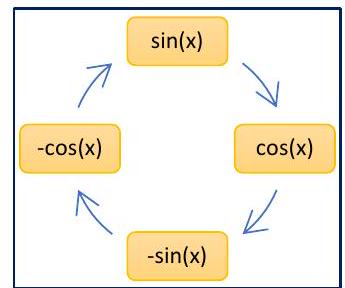
\includegraphics[scale=0.25]{Analysis1/zsf/Images/Differential/2024_01_20_7bfda6c084929ccc01ffg-05.jpg}
\end{center}














